% Options for packages loaded elsewhere
% Options for packages loaded elsewhere
\PassOptionsToPackage{unicode}{hyperref}
\PassOptionsToPackage{hyphens}{url}
%
\documentclass[
  ignorenonframetext,
  aspectratio=169,
  russian,
]{beamer}
\newif\ifbibliography
\usepackage{pgfpages}
\setbeamertemplate{caption}[numbered]
\setbeamertemplate{caption label separator}{: }
\setbeamercolor{caption name}{fg=normal text.fg}
\beamertemplatenavigationsymbolshorizontal
% remove section numbering
\setbeamertemplate{part page}{
  \centering
  \begin{beamercolorbox}[sep=16pt,center]{part title}
    \usebeamerfont{part title}\insertpart\par
  \end{beamercolorbox}
}
\setbeamertemplate{section page}{
  \centering
  \begin{beamercolorbox}[sep=12pt,center]{section title}
    \usebeamerfont{section title}\insertsection\par
  \end{beamercolorbox}
}
\setbeamertemplate{subsection page}{
  \centering
  \begin{beamercolorbox}[sep=8pt,center]{subsection title}
    \usebeamerfont{subsection title}\insertsubsection\par
  \end{beamercolorbox}
}
% Prevent slide breaks in the middle of a paragraph
\widowpenalties 1 10000
\raggedbottom
\AtBeginPart{
  \frame{\partpage}
}
\AtBeginSection{
  \ifbibliography
  \else
    \frame{\sectionpage}
  \fi
}
\AtBeginSubsection{
  \frame{\subsectionpage}
}
\usepackage{iftex}
\ifPDFTeX
  \usepackage[T1]{fontenc}
  \usepackage[utf8]{inputenc}
  \usepackage{textcomp} % provide euro and other symbols
\else % if luatex or xetex
  \usepackage{unicode-math} % this also loads fontspec
  \defaultfontfeatures{Scale=MatchLowercase}
  \defaultfontfeatures[\rmfamily]{Ligatures=TeX,Scale=1}
\fi
\usepackage{lmodern}

\ifPDFTeX\else
  % xetex/luatex font selection
\fi
% Use upquote if available, for straight quotes in verbatim environments
\IfFileExists{upquote.sty}{\usepackage{upquote}}{}
\IfFileExists{microtype.sty}{% use microtype if available
  \usepackage[]{microtype}
  \UseMicrotypeSet[protrusion]{basicmath} % disable protrusion for tt fonts
}{}


\usepackage{longtable,booktabs,array}
\newcounter{none} % for unnumbered tables
\usepackage{calc} % for calculating minipage widths
\usepackage{caption}
% Make caption package work with longtable
\makeatletter
\def\fnum@table{\tablename~\thetable}
\makeatother
\usepackage{graphicx}
\makeatletter
\newsavebox\pandoc@box
\newcommand*\pandocbounded[1]{% scales image to fit in text height/width
  \sbox\pandoc@box{#1}%
  \Gscale@div\@tempa{\textheight}{\dimexpr\ht\pandoc@box+\dp\pandoc@box\relax}%
  \Gscale@div\@tempb{\linewidth}{\wd\pandoc@box}%
  \ifdim\@tempb\p@<\@tempa\p@\let\@tempa\@tempb\fi% select the smaller of both
  \ifdim\@tempa\p@<\p@\scalebox{\@tempa}{\usebox\pandoc@box}%
  \else\usebox{\pandoc@box}%
  \fi%
}
% Set default figure placement to htbp
\def\fps@figure{htbp}
\makeatother



\ifLuaTeX
\usepackage[bidi=basic,shorthands=off,provide=*]{babel}
\else
\usepackage[bidi=default,shorthands=off,provide=*]{babel}
\fi
\ifLuaTeX
  \usepackage{selnolig} % disable illegal ligatures
\fi


\setlength{\emergencystretch}{3em} % prevent overfull lines

\providecommand{\tightlist}{%
  \setlength{\itemsep}{0pt}\setlength{\parskip}{0pt}}



 

\usepackage[]{csquotes}

%%% Load theme
\IfFileExists{beamerthemegotham.sty}{
  %%%% Full TeXlive
  \usetheme{gotham}
  \gothamset{
    numbering=totalframenumber,
    parttocframe default=off,
    sectiontocframe default=off,
    subsectiontocframe default=off,
    tocframe template=gotham bullet,
    % progressbar position=frametitle,
    progressbar position=foot,
  }
  \renewcommand{\gothamInstituteLogoSquare}[1][4ex]{%
    
\includegraphics[height=##1]{_resources/image/logo_rudn-inverted.png}
  }
  % \renewcommand{\gothamtitlepagelogo}[1][4ex]{%
  %   
\includegraphics[height=##1]{_resources/image/logo_rudn.png}
  % }
}{%
  %%%% TinyTeX
  \usepackage{libertine}
  %%%% https://deic.uab.cat/~iblanes/beamer_gallery/
  \usetheme{Madrid}
}
\makeatletter
\@ifpackageloaded{caption}{}{\usepackage{caption}}
\AtBeginDocument{%
\ifdefined\contentsname
  \renewcommand*\contentsname{Содержание}
\else
  \newcommand\contentsname{Содержание}
\fi
\ifdefined\listfigurename
  \renewcommand*\listfigurename{Список иллюстраций}
\else
  \newcommand\listfigurename{Список иллюстраций}
\fi
\ifdefined\listtablename
  \renewcommand*\listtablename{Список таблиц}
\else
  \newcommand\listtablename{Список таблиц}
\fi
\ifdefined\figurename
  \renewcommand*\figurename{Рисунок}
\else
  \newcommand\figurename{Рисунок}
\fi
\ifdefined\tablename
  \renewcommand*\tablename{Таблица}
\else
  \newcommand\tablename{Таблица}
\fi
}
\@ifpackageloaded{float}{}{\usepackage{float}}
\floatstyle{ruled}
\@ifundefined{c@chapter}{\newfloat{codelisting}{h}{lop}}{\newfloat{codelisting}{h}{lop}[chapter]}
\floatname{codelisting}{Список}
\newcommand*\listoflistings{\listof{codelisting}{Листинги}}
\makeatother
\makeatletter
\makeatother
\makeatletter
\@ifpackageloaded{caption}{}{\usepackage{caption}}
\@ifpackageloaded{subcaption}{}{\usepackage{subcaption}}
\makeatother

\usepackage{bookmark}
\IfFileExists{xurl.sty}{\usepackage{xurl}}{} % add URL line breaks if available
\urlstyle{same}
% fallback for those not using the hyperref driver hyperxmp:
\makeatletter
\@ifundefined{xmpquote}{\newcommand{\xmpquote}[1]{#1}}{}
\makeatother
\hypersetup{
  pdftitle={Презентация по лабораторной работе №1},
  pdfauthor={Люпп Софья Романовна},
  pdflang={ru-RU},
  hidelinks,
  pdfcreator={LaTeX via pandoc}}


\title{\texorpdfstring{Презентация по лабораторной работе
№1}{Презентация по лабораторной работе №1}}
\subtitle{\texorpdfstring{Подготовка стенда и установка
Julia}{Подготовка стенда и установка Julia}}
\author{Люпп Софья Романовна}
\date{2026-09-12}

\begin{document}
\frame{\titlepage}

\renewcommand*\contentsname{Содержание}
\begin{frame}[allowframebreaks]
  \frametitle{Содержание}
  \setcounter{tocdepth}{2}
  \tableofcontents
\end{frame}
\setcounter{tocdepth}{2}
\tableofcontents
}

\section{Информация}\label{ux438ux43dux444ux43eux440ux43cux430ux446ux438ux44f}

\begin{frame}{Докладчик}
\protect\phantomsection\label{ux434ux43eux43aux43bux430ux434ux447ux438ux43a}
\begin{columns}[c]
\begin{column}{0.7\linewidth}
\begin{itemize}
\tightlist
\item
  Люпп Софья Романовна
\item
  студентка группы НКНбд-01-23
\item
  кафедра теории вероятностей и кибербезопасности
\item
  Российский университет дружбы народов им. П. Лумумбы
\item
  {[}1132236039@rudn.ru{]}
\item
  \url{https://github.com/srluipp}
\end{itemize}
\end{column}

\begin{column}{0.3\linewidth}
\end{column}
\end{columns}
\end{frame}

\section{Вводная
часть}\label{ux432ux432ux43eux434ux43dux430ux44f-ux447ux430ux441ux442ux44c}

\begin{frame}{Актуальность}
\protect\phantomsection\label{ux430ux43aux442ux443ux430ux43bux44cux43dux43eux441ux442ux44c}
Julia актуальна как инструмент для научных вычислений, финансового
моделирования, искусственного интеллекта, вычислений в области инженерии
и физики, благодаря своей высокой производительности, простоте
синтаксиса и гибкости в работе с массивами и параллельным
программированием
\end{frame}

\begin{frame}{Объект и предмет исследования}
\protect\phantomsection\label{ux43eux431ux44aux435ux43aux442-ux438-ux43fux440ux435ux434ux43cux435ux442-ux438ux441ux441ux43bux435ux434ux43eux432ux430ux43dux438ux44f}
Julia является обьектом и предметом исследования
\end{frame}

\begin{frame}{Цели и задачи}
\protect\phantomsection\label{ux446ux435ux43bux438-ux438-ux437ux430ux434ux430ux447ux438}
Цель данной лабораторной работы - приобретение практических навыков
работы с системой управления версиями Git, языком программирования
Julia.
\end{frame}

\section{Выполнение лабораторной
работы}\label{ux432ux44bux43fux43eux43bux43dux435ux43dux438ux435-ux43bux430ux431ux43eux440ux430ux442ux43eux440ux43dux43eux439-ux440ux430ux431ux43eux442ux44b}

\begin{frame}{Выполнение лабораторной работы}
Начинаю с подготовки и настройки рабочего пространства (установка git),
котоая у меня уже была, перехожу к созданию ключей ssh
(рис.~\ref{fig-001}).

\begin{figure}

\centering{

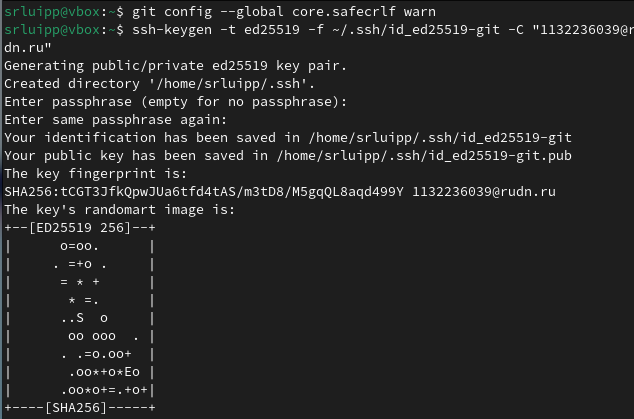
\includegraphics[width=0.7\linewidth,height=\textheight,keepaspectratio]{image/1.png}

}

\caption{\label{fig-001}git}

\end{figure}%
\end{frame}

\begin{frame}{Настройка ключей ssh}
\protect\phantomsection\label{ux43dux430ux441ux442ux440ux43eux439ux43aux430-ux43aux43bux44eux447ux435ux439-ssh}
(рис.~\ref{fig-002})

\begin{figure}

\centering{

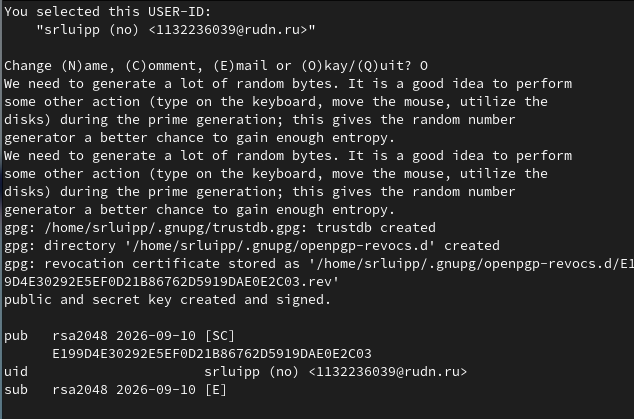
\includegraphics[width=0.7\linewidth,height=\textheight,keepaspectratio]{image/2.png}

}

\caption{\label{fig-002}ssh}

\end{figure}%
\end{frame}

\begin{frame}{Настройка ключей ssh}
\protect\phantomsection\label{ux43dux430ux441ux442ux440ux43eux439ux43aux430-ux43aux43bux44eux447ux435ux439-ssh-1}
(рис.~\ref{fig-003})

\begin{figure}

\centering{

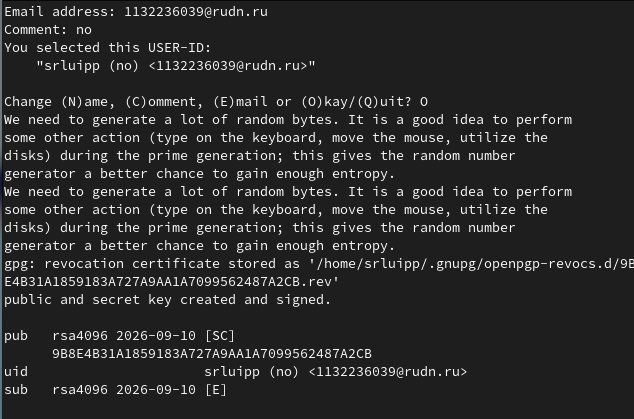
\includegraphics[width=0.7\linewidth,height=\textheight,keepaspectratio]{image/3.png}

}

\caption{\label{fig-003}ssh}

\end{figure}%
\end{frame}

\begin{frame}{Настройка ключей ssh}
\protect\phantomsection\label{ux43dux430ux441ux442ux440ux43eux439ux43aux430-ux43aux43bux44eux447ux435ux439-ssh-2}
(рис.~\ref{fig-004})

\begin{figure}

\centering{

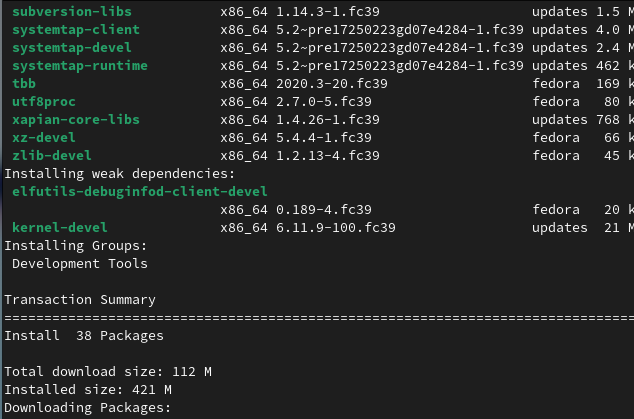
\includegraphics[width=0.7\linewidth,height=\textheight,keepaspectratio]{image/4.png}

}

\caption{\label{fig-004}ssh}

\end{figure}%
\end{frame}

\begin{frame}{libxcrypt-compact}
\protect\phantomsection\label{libxcrypt-compact}
Устанавливаю библиотеку libxcrypt-compact(рис.~\ref{fig-005}).

\begin{figure}

\centering{

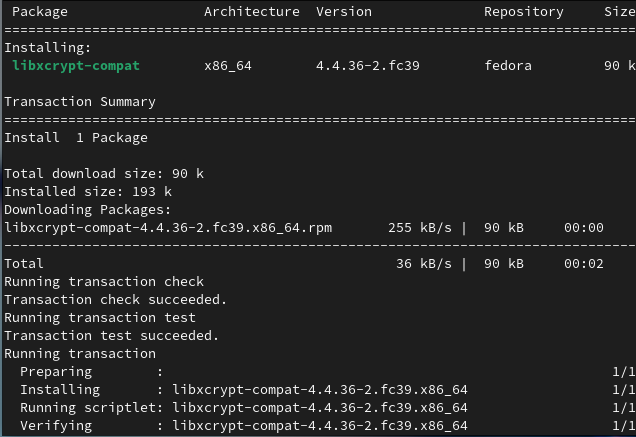
\includegraphics[width=0.7\linewidth,height=\textheight,keepaspectratio]{image/5.png}

}

\caption{\label{fig-005}libxcrypt-compact}

\end{figure}%
\end{frame}

\begin{frame}{quarto}
\protect\phantomsection\label{quarto}
Устанавливаю quarto (рис.~\ref{fig-006})

\begin{figure}

\centering{

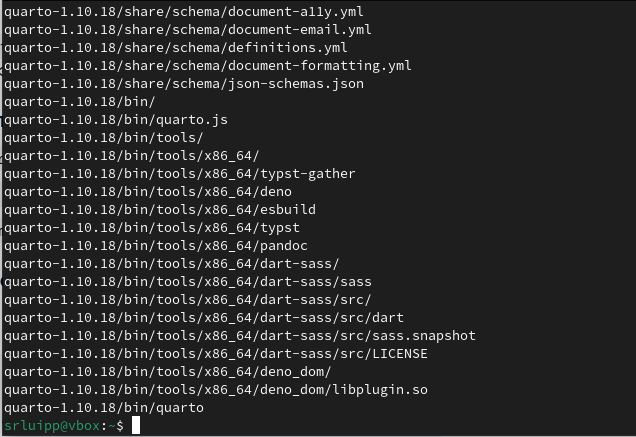
\includegraphics[width=0.7\linewidth,height=\textheight,keepaspectratio]{image/6.png}

}

\caption{\label{fig-006}quarto}

\end{figure}%
\end{frame}

\begin{frame}{quarto}
\protect\phantomsection\label{quarto-1}
(рис. Рисунок~\ref{fig-007}{]})

\begin{figure}

\centering{

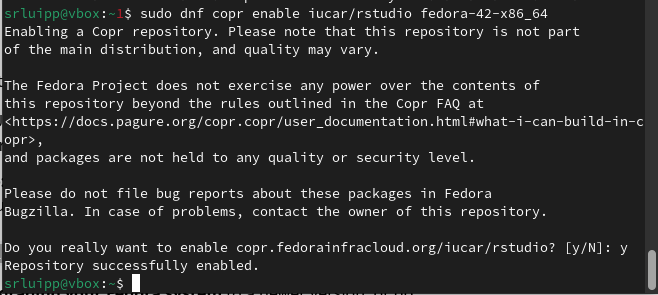
\includegraphics[width=0.7\linewidth,height=\textheight,keepaspectratio]{image/7.png}

}

\caption{\label{fig-007}quarto}

\end{figure}%
\end{frame}

\begin{frame}{}
\protect\phantomsection\label{section}
Устанавливаю node.js (рис.~\ref{fig-008}).

\begin{figure}

\centering{

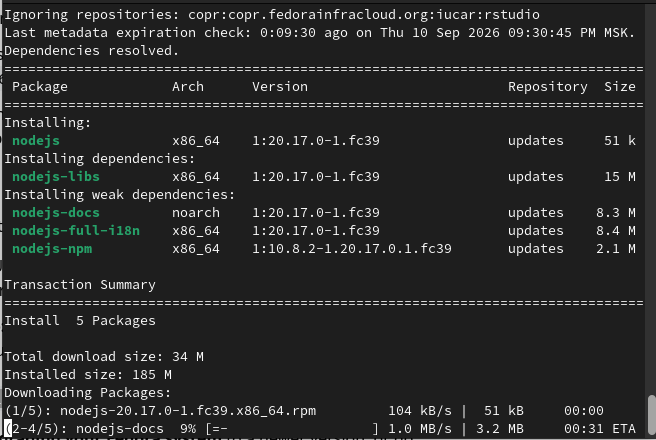
\includegraphics[width=0.7\linewidth,height=\textheight,keepaspectratio]{image/8.png}

}

\caption{\label{fig-008}nodejs}

\end{figure}%
\end{frame}

\begin{frame}{}
\protect\phantomsection\label{section-1}
Устанавливаю pnpm(рис.~\ref{fig-009}).

\begin{figure}

\centering{

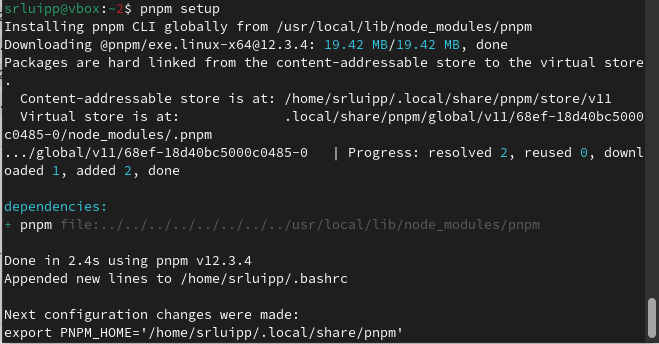
\includegraphics[width=0.7\linewidth,height=\textheight,keepaspectratio]{image/9.png}

}

\caption{\label{fig-009}pnpm}

\end{figure}%

Устанавливаю pnpm commitzens (рис.~\ref{fig-010})

\begin{figure}

\centering{

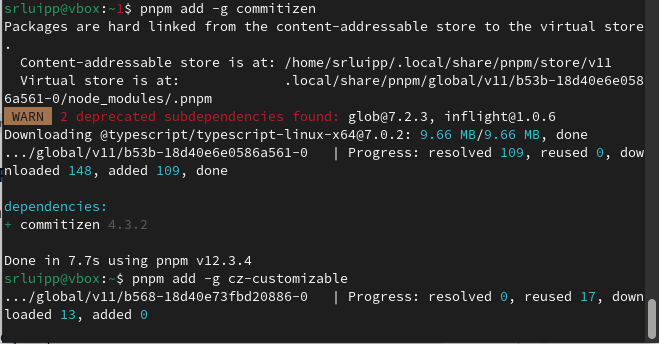
\includegraphics[width=0.7\linewidth,height=\textheight,keepaspectratio]{image/10.png}

}

\caption{\label{fig-010}pnpm}

\end{figure}%
\end{frame}

\begin{frame}{}
\protect\phantomsection\label{section-2}
(рис.~\ref{fig-011})

\begin{figure}

\centering{

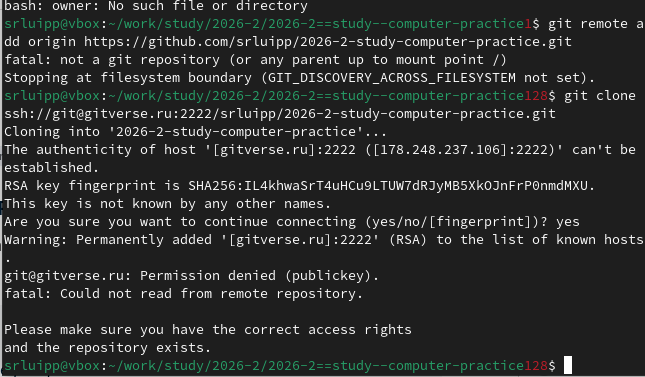
\includegraphics[width=0.7\linewidth,height=\textheight,keepaspectratio]{image/11.png}

}

\caption{\label{fig-011}pnpm}

\end{figure}%
\end{frame}

\begin{frame}{}
\protect\phantomsection\label{section-3}
Клонирую репозиторий в GitVerse(рис.~\ref{fig-012})

\begin{figure}

\centering{

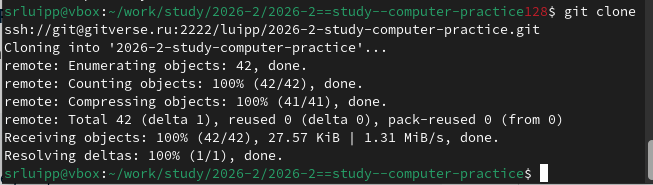
\includegraphics[width=0.7\linewidth,height=\textheight,keepaspectratio]{image/12.png}

}

\caption{\label{fig-012}git clone}

\end{figure}%
\end{frame}

\begin{frame}{}
\protect\phantomsection\label{section-4}
(рис.~\ref{fig-013})

\begin{figure}

\centering{

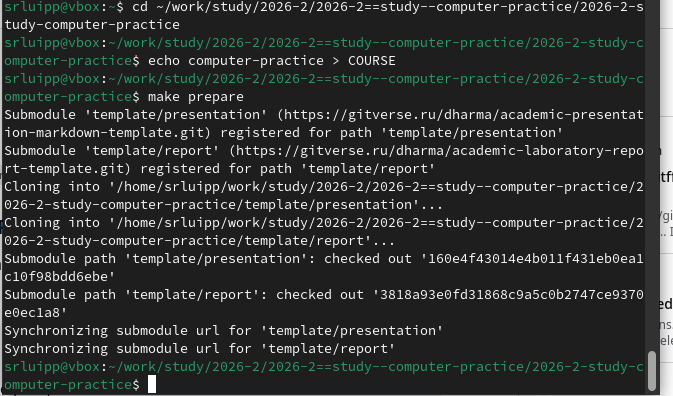
\includegraphics[width=0.7\linewidth,height=\textheight,keepaspectratio]{image/13.png}

}

\caption{\label{fig-013}git clone}

\end{figure}%
\end{frame}

\begin{frame}{}
\protect\phantomsection\label{section-5}
Произвожу команды make и пушу на гит(рис.~\ref{fig-014})

\begin{figure}

\centering{

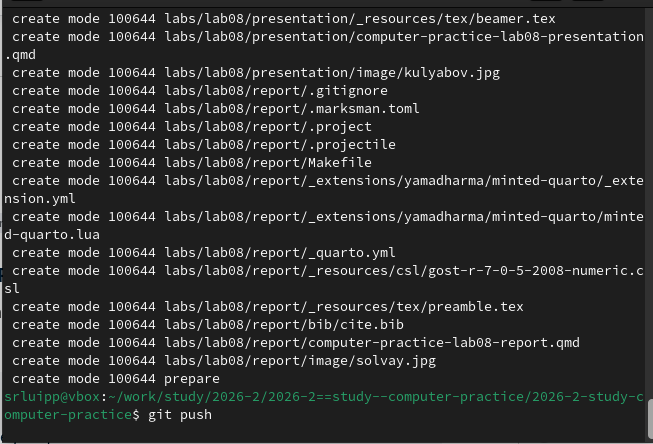
\includegraphics[width=0.7\linewidth,height=\textheight,keepaspectratio]{image/14.png}

}

\caption{\label{fig-014}make}

\end{figure}%
\end{frame}

\begin{frame}{}
\protect\phantomsection\label{section-6}
(рис.~\ref{fig-015})

\begin{figure}

\centering{

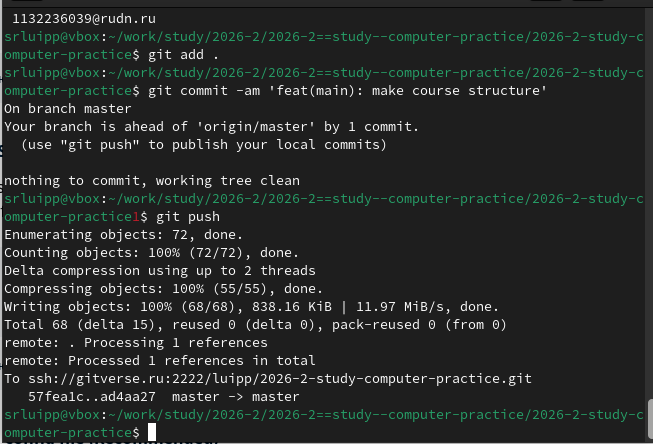
\includegraphics[width=0.7\linewidth,height=\textheight,keepaspectratio]{image/15.png}

}

\caption{\label{fig-015}make and push}

\end{figure}%
\end{frame}

\begin{frame}{}
\protect\phantomsection\label{section-7}
Теперь необходимо установить и распаковать gitflow (рис.~\ref{fig-016})

\begin{figure}

\centering{

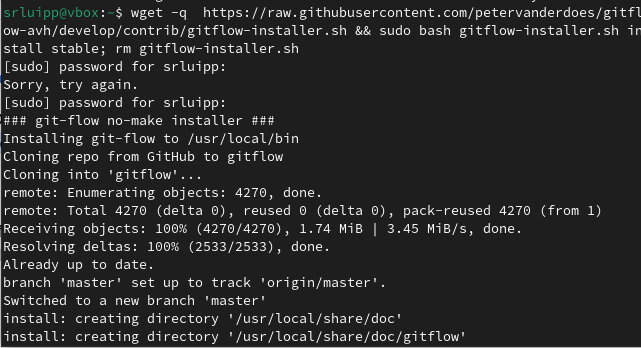
\includegraphics[width=0.7\linewidth,height=\textheight,keepaspectratio]{image/16.png}

}

\caption{\label{fig-016}gitflow}

\end{figure}%
\end{frame}

\begin{frame}{}
\protect\phantomsection\label{section-8}
(рис.~\ref{fig-017})

\begin{figure}

\centering{

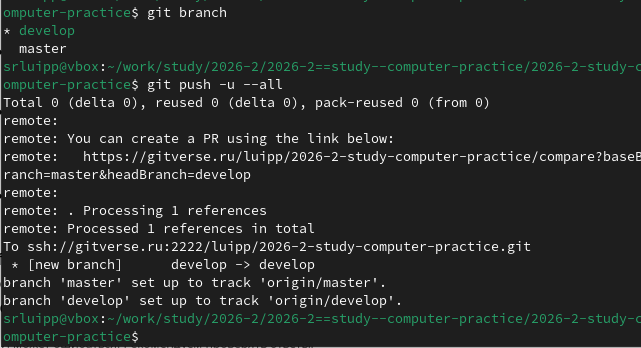
\includegraphics[width=0.7\linewidth,height=\textheight,keepaspectratio]{image/17.png}

}

\caption{\label{fig-017}gitflow}

\end{figure}%
\end{frame}

\begin{frame}{}
\protect\phantomsection\label{section-9}
Настройка branches (рис.~\ref{fig-018}).

\begin{figure}

\centering{

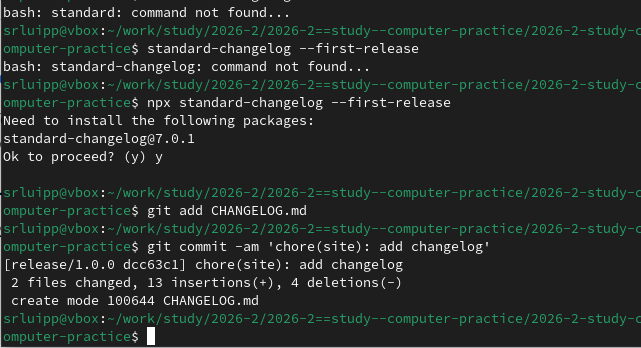
\includegraphics[width=0.7\linewidth,height=\textheight,keepaspectratio]{image/18.png}

}

\caption{\label{fig-018}branches}

\end{figure}%
\end{frame}

\begin{frame}{}
\protect\phantomsection\label{section-10}
Checking the branches (рис.~\ref{fig-019})

\begin{figure}

\centering{

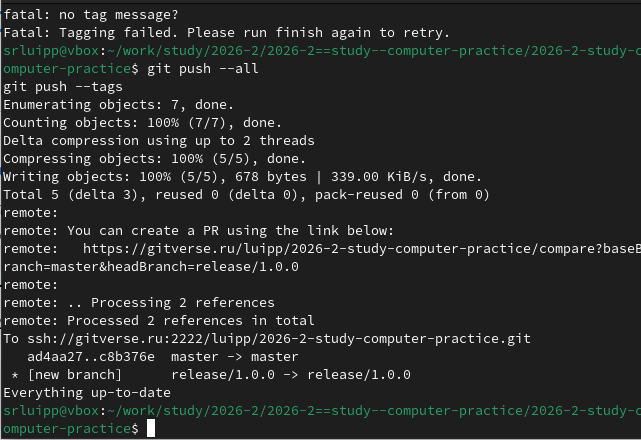
\includegraphics[width=0.7\linewidth,height=\textheight,keepaspectratio]{image/19.png}

}

\caption{\label{fig-019}branches2}

\end{figure}%
\end{frame}

\begin{frame}{}
\protect\phantomsection\label{section-11}
(рис.~\ref{fig-020})

\begin{figure}

\centering{

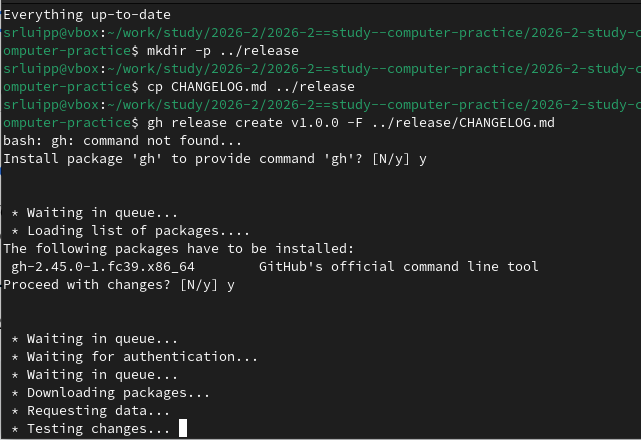
\includegraphics[width=0.7\linewidth,height=\textheight,keepaspectratio]{image/20.png}

}

\caption{\label{fig-020}branches3}

\end{figure}%
\end{frame}

\begin{frame}{}
\protect\phantomsection\label{section-12}
Устанавливаю пакет julia (рис.~\ref{fig-021}).

\begin{figure}

\centering{

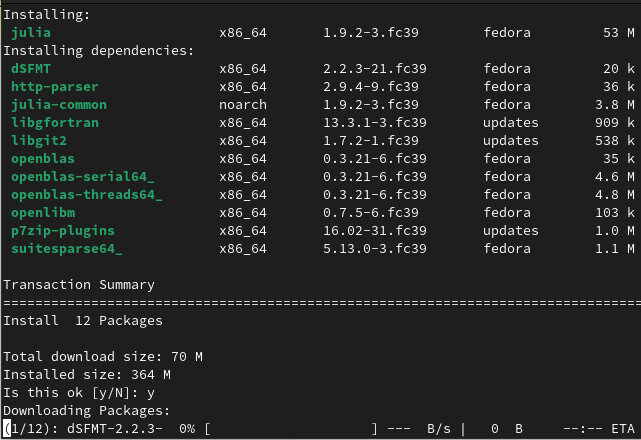
\includegraphics[width=0.7\linewidth,height=\textheight,keepaspectratio]{image/21.png}

}

\caption{\label{fig-021}julia}

\end{figure}%
\end{frame}

\begin{frame}{}
\protect\phantomsection\label{section-13}
Устанавливаю необходимые дополнения для julia (рис.~\ref{fig-022})

\begin{figure}

\centering{

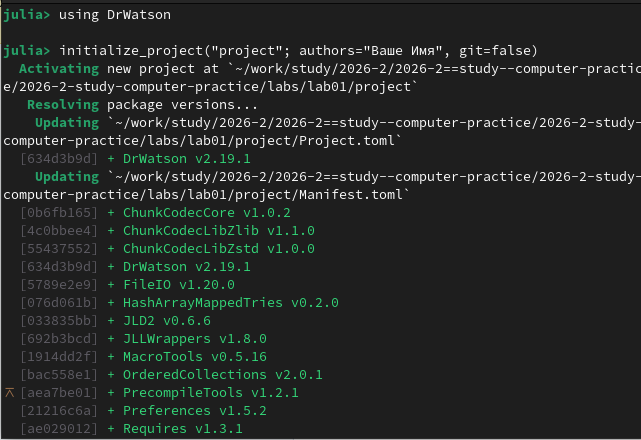
\includegraphics[width=0.7\linewidth,height=\textheight,keepaspectratio]{image/22.png}

}

\caption{\label{fig-022}julia}

\end{figure}%
\end{frame}

\begin{frame}{}
\protect\phantomsection\label{section-14}
(рис.~\ref{fig-023})

\begin{figure}

\centering{

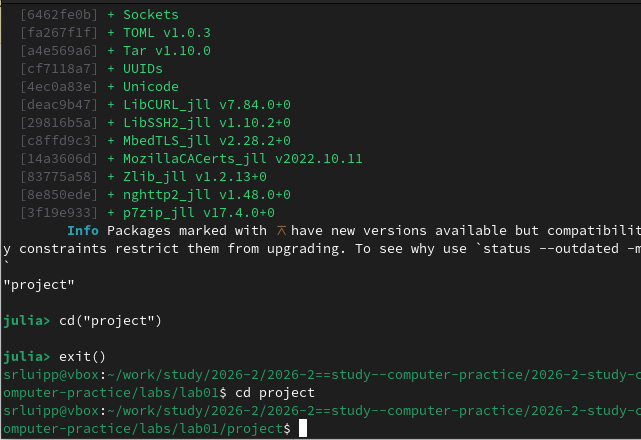
\includegraphics[width=0.7\linewidth,height=\textheight,keepaspectratio]{image/23.png}

}

\caption{\label{fig-023}julia}

\end{figure}%
\end{frame}

\begin{frame}{}
\protect\phantomsection\label{section-15}
(рис.~\ref{fig-024})

\begin{figure}

\centering{

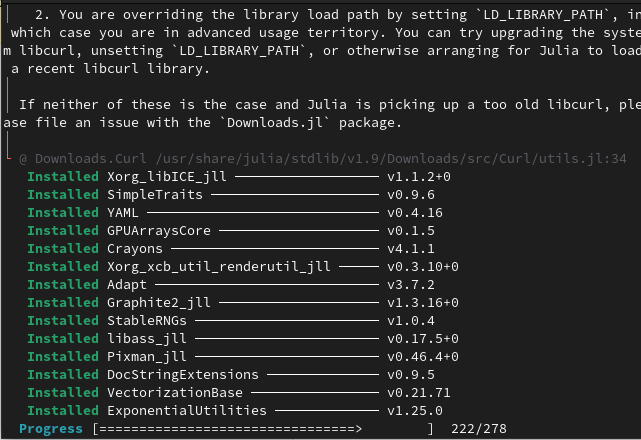
\includegraphics[width=0.7\linewidth,height=\textheight,keepaspectratio]{image/24.png}

}

\caption{\label{fig-024}julia}

\end{figure}%
\end{frame}

\section{Выводы}\label{ux432ux44bux432ux43eux434ux44b}

\begin{frame}{Выводы}
В ходе лабораторной работы я приобрела практические навыки работы с
системой управления версиями Git, языком программирования Julia.
\end{frame}




\end{document}
